\begin{figure}[H]
    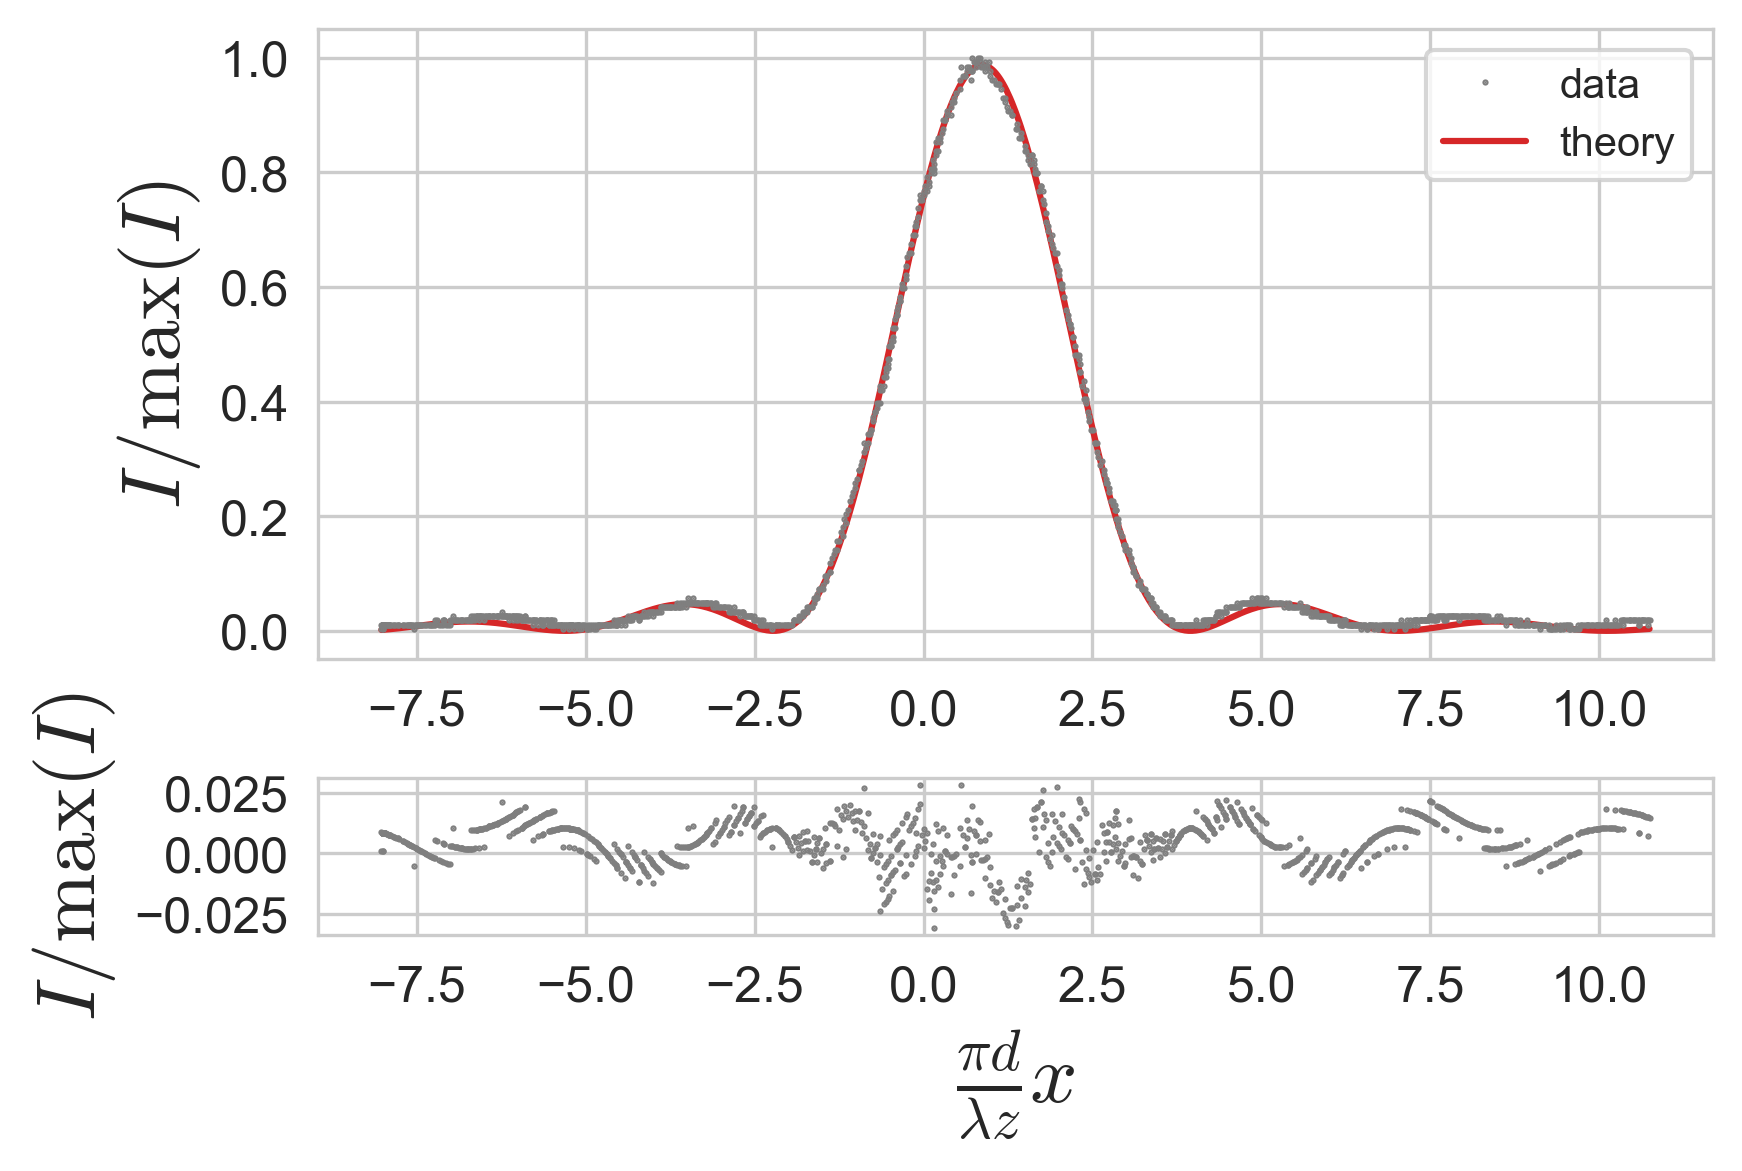
\includegraphics[width=0.9\columnwidth]{figures/single slit interference with 0.04mm width.png}
    \caption{a comparison of the interference pattern of a 0.04 mm with slit with the theoretical prediction.\\
    Note the pattern within the tails of the residual graph showing presence of a secondary effect as demonstrated with
    greater clarity by \ref{fig:single slit interference with 0.04mm not best fit but better tails}}
    \label{fig:single slit interference with 0.04mm width},($\sigma\sim0.0086$)
\end{figure}